\chapter{Конструкторская часть}
\label{cha:design}

В данном разделе будет рассмотрены схемы.

На рис. \ref{ref:d0} показана схема алгоритма главного потока.

\begin{figure}[ht!]
	\centering{
		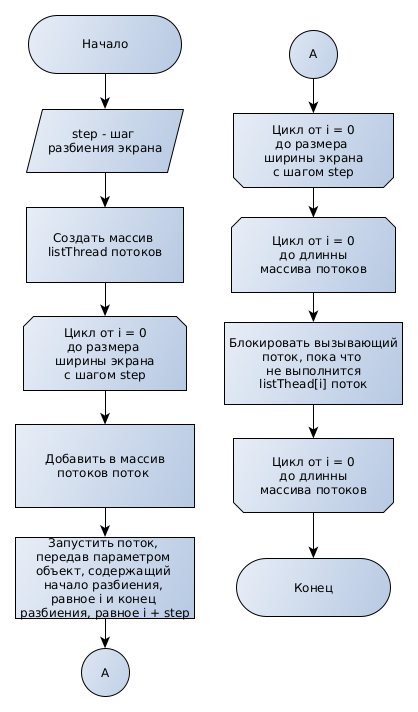
\includegraphics[width=0.8\textwidth]{d4.png}
		\caption{Схема алгоритма главного потока}
		\label{ref:d0}}
\end{figure}

На рис. \ref{ref:d1} показана схема работы потока, который разбивает
экран вертикально.

\begin{figure}[ht!]
	\centering{
		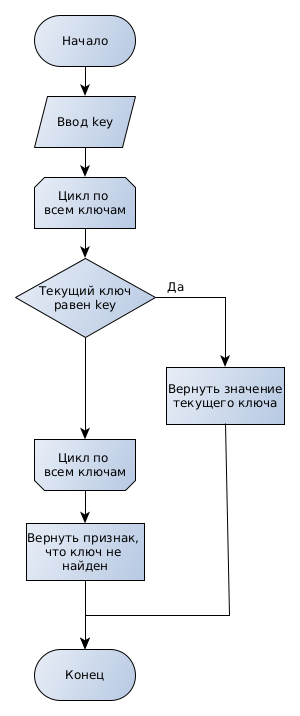
\includegraphics[width=0.8\textwidth]{d1.png}
		\caption{Вертикальное разбиение экрана}
		\label{ref:d1}}
\end{figure}

На рис. \ref{ref:d2} показана схема работы потока, который разбивает
экран горизонтально.

\begin{figure}[ht!]
	\centering{
		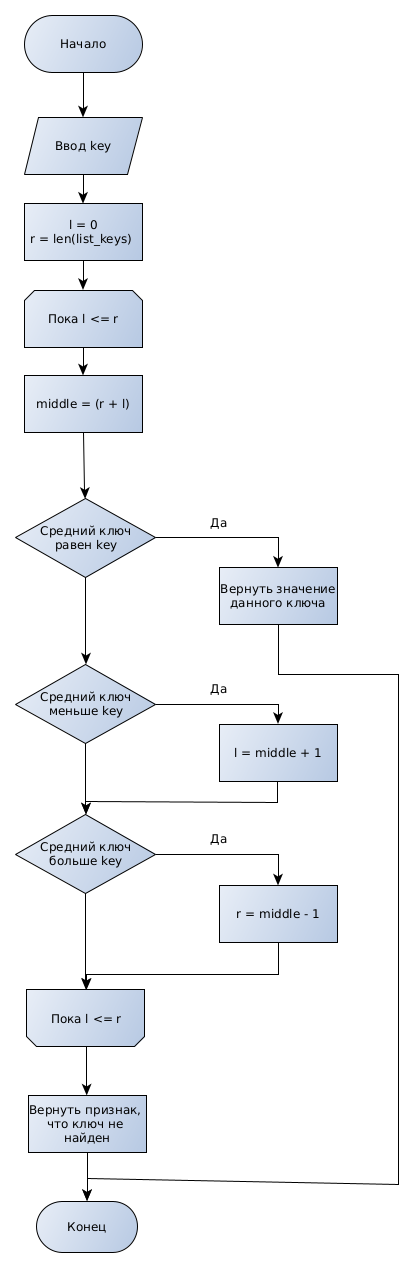
\includegraphics[width=0.8\textwidth]{d2.png}
		\caption{Горизонтальное разбиение экрана}
		\label{ref:d2}}
\end{figure}

На рис. \ref{ref:d3} показана схема однопоточного алгоритма трассировки
лучей.

\begin{figure}[ht!]
	\centering{
		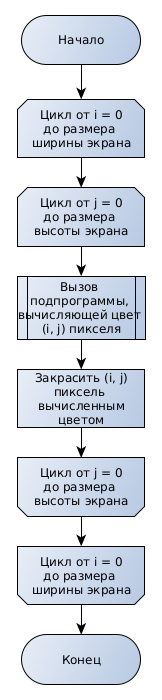
\includegraphics[width=0.3\textwidth]{d3.png}
		\caption{Однопоточная трассировка лучей}
		\label{ref:d3}}
\end{figure}



\section{Вывод}

В данном разделе были рассмотрены схемы однопоточной (рис. \ref{ref:d3}) и многопоточной
(рис. \ref{ref:d0} - \ref{ref:d2}) реализации алгоритма обратной трассировки лучей






